\frontmatter
%\let\indexORI\index% sauvegarde de la définition initiale
%\renewcommand{\index}[1]{\indexORI{##1|textsc}}
%\fancyfoot{}
%\fancyhead[LE,RO]{\textsc{\thepage}}

\chapter{Avant-propos à vocation introductive}
\epigraph{Dire des idioties, de nos jours où tout le monde réfléchit profondément, c'est le seul moyen de prouver qu'on a une pensée libre et indépendante.}{\BV}
\vfill
\pagebreak

L'auteur souhaite la bienvenue au lecteur. Qu'il attache sa ceinture,
se serve un bon verre de scotch\footnote{Ou de café, thé, ou tout autre
boisson ayant ses faveurs; l'auteur n'est pas regardant.}, place un
disque de jazz\footnote{L'auteur recommande du Duke \bsc{Ellington}, 
Miles \bsc{Davis}, ou encore Bix \bsc{Beideiderbeckeke}. Il est envisageable de
passer des compositions de \BV\ lui-même, ou de Henri \bsc{Salvador}.}
sur le \emph{pick-up}\footnote{À défaut de \emph{pick-up},
le lecteur peut utiliser une platine CD, voire une liste de lecture
stockée sur ordinateur.}
il s'apprête à découvrir (peut-être !), à comprendre (en partie) le
personnage extravagant qu'a été \BV, et comment, \nb{50} ans après
sa mort, il est devenu incontournable dans le paysage culturel français.

Cependant, qu'il soit averti: ce document n'a pas vocation à être exhaustif
--- il faudrait être prétentieux pour cela, ce que ce document n'est pas
non plus. Des ouvrages, rédigés par des gens plus compétents et renseignés
que votre serviteur, tendent vers ce but.
Ce document, donc, se veut un espèce d'hommage (fort modeste) à
Boris\footnote{Le lecteur excusera la familiarité. C'est qu'à force de
documentation, l'auteur et le sujet ont eu le temps de faire connaissance.},
en présentant des aspects de sa vie et de son \oe{}uvre méritant
que l'on s'y attarde, quand ils ne forcent pas tout bonnement le respect.
À ce titre, il est illustré de nombreuses images et agrémenté
de citations. Le lecteur pourra ainsi se faire son idée propre. De plus, 
certains élément peuvent être inexacts, voire erronés. Il ne
s'agit pas là d'une marque de mauvaise volonté de la part de l'auteur. Tout
au plus peut on y voir de l'ignorance. Ou de l'imagination. Allez savoir.
De nos jours, on est plus sûr de rien !


Passons maintenant à un ton plus personnel: comment l'auteur à
 découvert \BV, la genèse de ce document\ldots tout ce qui rend ce projet «personnel», finalement.
Quoi de mieux qu'une \emph{interview} pour cela ?
L'auteur s'est donc armé d'un magnétophone, a pris rendez-vous avec lui-même
et choisi un miroir de la meilleure facture pour immortaliser le dialogue suivant:

\begin{quotation}
- Bonjour M. Lizé. Je vous remercie de bien vouloir répondre à mes questions.

- Bonjour. Il n'y a pas de quoi, voyons ! Et puis, tutoyons-nous et appellons-nous
Raphaël. On est entre soi, tout de même !

- Très bien Raphaël. Je vais d'abord vous\ldots enfin {\bf te} demander comment
j'ai\ldots heu {\bf tu}\footnote{L'autointerview est un exercice des plus difficiles, auquel, hélas,
l'auteur n'est pas rompu.} as découvert \BV\ldots

- Excellente question ! J'ai fait la connaissance de \BV\ petit. Mes parents
possédaient --- et possèdent toujours ! --- un disque vinyle
regroupant ses meilleurs succès --- le voilà. \footnote{Il s'agit en fait de l'édition «Album Or» de l'album \emph{Le déserteur},
publié par Philips sous le numéro
de catalogue \nb{9101 268} en \nb{1975}. Voir fig. \ref{or}}. Ce disque m'attirait:
tu vois, la pochette est dorée et représente un monsieur à l'air sympathique,
souriant de toute ses dents. Au dos, les noms des chansons plus ou moins farfelus\ldots
et regarde à l'intérieur: les paroles étant tout ce qu'il y a de plus comique.
Je demandais souvent à mon père de passer ce disque. Écoutons le, tu veux bien ?

\emph{J'acquiesce. Il se dirige vers
la platine vinyle, y place le disque. Tout est prêt, il l'aurait probablement passé même sans me demander mon accord !\\
Voici la liste des pistes, dans l'ordre:
\begin{multicols}{2}
Face A:
\begin{itemize}
\item[A\nb{1}] Les joyeux bouchers 		
\item[A\nb{2}] Cinématographe 		
\item[A\nb{3}] La java des bombes atomiques 		
\item[A\nb{4}] Je bois 		
\item[A\nb{5}] Le petit commerce 		
\end{itemize}
\el
Face B:
\begin{itemize}
\item[B\nb{1}]J'suis snob 		
\item[B\nb{2}] Complainte du progrès «Les Arts Ménagers» 		
\item[B\nb{3}] On est pas là pour se faire eng... 		
\item[B\nb{4}] Bourrée de complexes 		
\item[B\nb{5}] Le déserteur 		
\end{itemize}
\end{multicols}
}

- Ça rappelle des souvenirs, hein ? Et ça n'a pas pris une ride !

- Effectivement ! J'apprécie également beaucoup cet album ! Mais, si certains
airs sont purement comiques, comme \emph{J'suis snob}, \emph{Je bois} ou l'invraisemblable
\emph{Complainte du progrès}, il y a également des textes très sérieux !

- Bien entendu, je ne comprenais pas alors tout le sens de certaines
chansons, m'arrêtant à l'époque au ton humoristique du texte. Maintenant, avec le recul,
les subtilités parviennent à mon cerveau lent.
\begin{figure}[hbt]
\centering
\begin{subfigure}[b]{.45\textwidth}
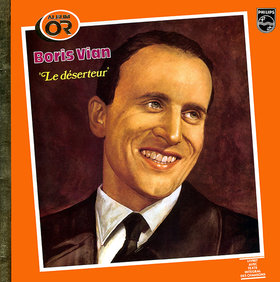
\includegraphics[width=\textwidth]{\PIXPATH/or}
\caption{Le vinyle de \BV}
\label{or}
\end{subfigure}\quad%
\begin{subfigure}[b]{.45\textwidth}
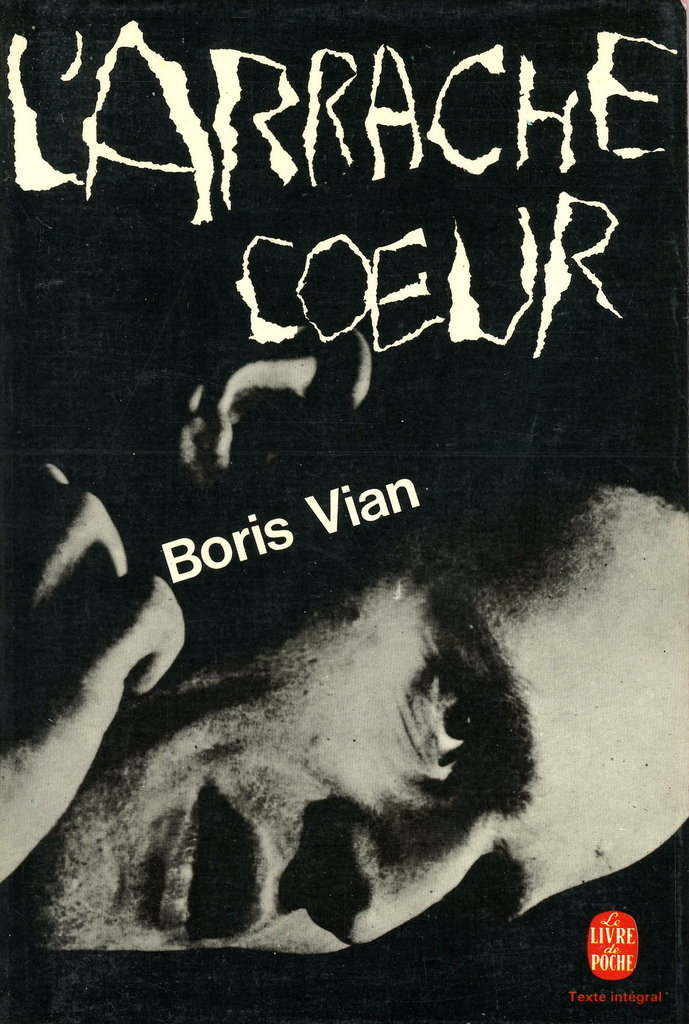
\includegraphics[width=.8\textwidth]{\PIXPATH/arrache}
\caption{\emph{L'arrache c\oe{}ur}, édition Livre de Poche de \nb{1977}. Illustration de Pierre \bsc{Faucheux}. Brrrrr.}
\label{arco}
\end{subfigure}
\caption{Mes premiers contacts avec Vian.}
\end{figure}

- C'est donc l'auteur interprète que tu as découvert en premier.

- Oui ! Mais, à l'époque, avide de lecture, j'écumais la bibliothèque de mes parents. 
Je suis en suite tombé, un jour, sur une édition
de \emph{L'arrache c\oe{}ur}. Encore jeune, j'ai été marqué par
le titre particulièrement violent. L'illustration de cette édition,
que voilà ( \emph{note de l'auteur: fig. \ref{arco}}), a participé à cette impression. J'ai
donc laissé de côté pour un moment l'écrivain. J'ai bien sûr
entendu parler de ses autres livres, en particulier de
\emph{L'écume des jours}, mais à chaque fois me revenait
l'image de \emph{L'arrache c\oe{}ur}, et je n'ai pas cherché
plus loin.

- Je te comprends. Et ensuite ?

- Ce n'est que bien plus tard que ma curiosité à été ravivée\ldots
je ne sais plus exactement quand ni par quoi. J'avais toujours
en mémoire ses chansons, si drôles.
Toujours est-il
que je me suis retrouvé à lire --- avec délectation ! --- ses romans
de jeunesse: \emph{Vercoquin et le plancton}, \emph{Trouble dans
les Andains}, \emph{Comte de fées à l'usage des moyennes personnes}\ldots
réédités au sein du premier tome de l'intégrale des ses \oe{}uvres
écrites\footnote{\emph{\OE{}uvres de Boris Vian}, tome \nb{1}, chez Fayard.}.
La préface, de Noël \bsc{Arnaud}, excellente, m'a donné l'envie d'en apprendre plus,
et de là est née l'idée de sujet de ce PPH.
Ensuite, j'ai lu \emph{J'irai cracher}, \emph{L'écume}, \emph{L'herbe rouge}\ldots quel talent !

- C'était donc cela ! Cela a vraiment du se révéler intéressant. Une dernière question cependant:
as-tu rencontré des difficultés lors de la réalisation de ce PPH ?

- Eh bien\ldots je dois dire que ce bougre de Boris n'a pas facilité la tâche
de ceux qui voudraient connaître sa vie ! Ça part dans tous les sens ! Il a tout fait, tout !
Et puis surtout, il a tout fait en même temps !
(\emph{il attrape un carnet et des crayons, puis, d'une main habile sinon experte, s'exprima 
durant quelques instants sur le support encore vierge, et me tendis l'objet.
Le contenu est reproduit fig. \ref{carnet}}).

- Ah oui, effectivement\ldots mais comment as-tu exploré cela ?

- Je me suis beaucoup servi de l'exceptionnel ouvrage --- vraiment bien documenté ! --- de Noël \bsc{Arnaud}\ldots
\emph{Les vies parallèles de Boris Vian}\ldots qu'il aurait dû nommer
\emph{Les vies qui-se-coupent-dans-tous-les-sens de Boris Vian}, si tu veux mon avis !
Enfin, c'est donc ce livre qui m'a guidé et m'a permis de choisir de quoi j'allais traiter
dans mon dossier.

\emph{Sur ces bonnes paroles, nous nous fûmes nous promener dans les bois,
profitant du fais que le loup n'y étais pas. En effet, y eut-il été,
eûmes-nous fini dévorés sans coup faire rire !}
 
\end{quotation}

\begin{figure}
\centering
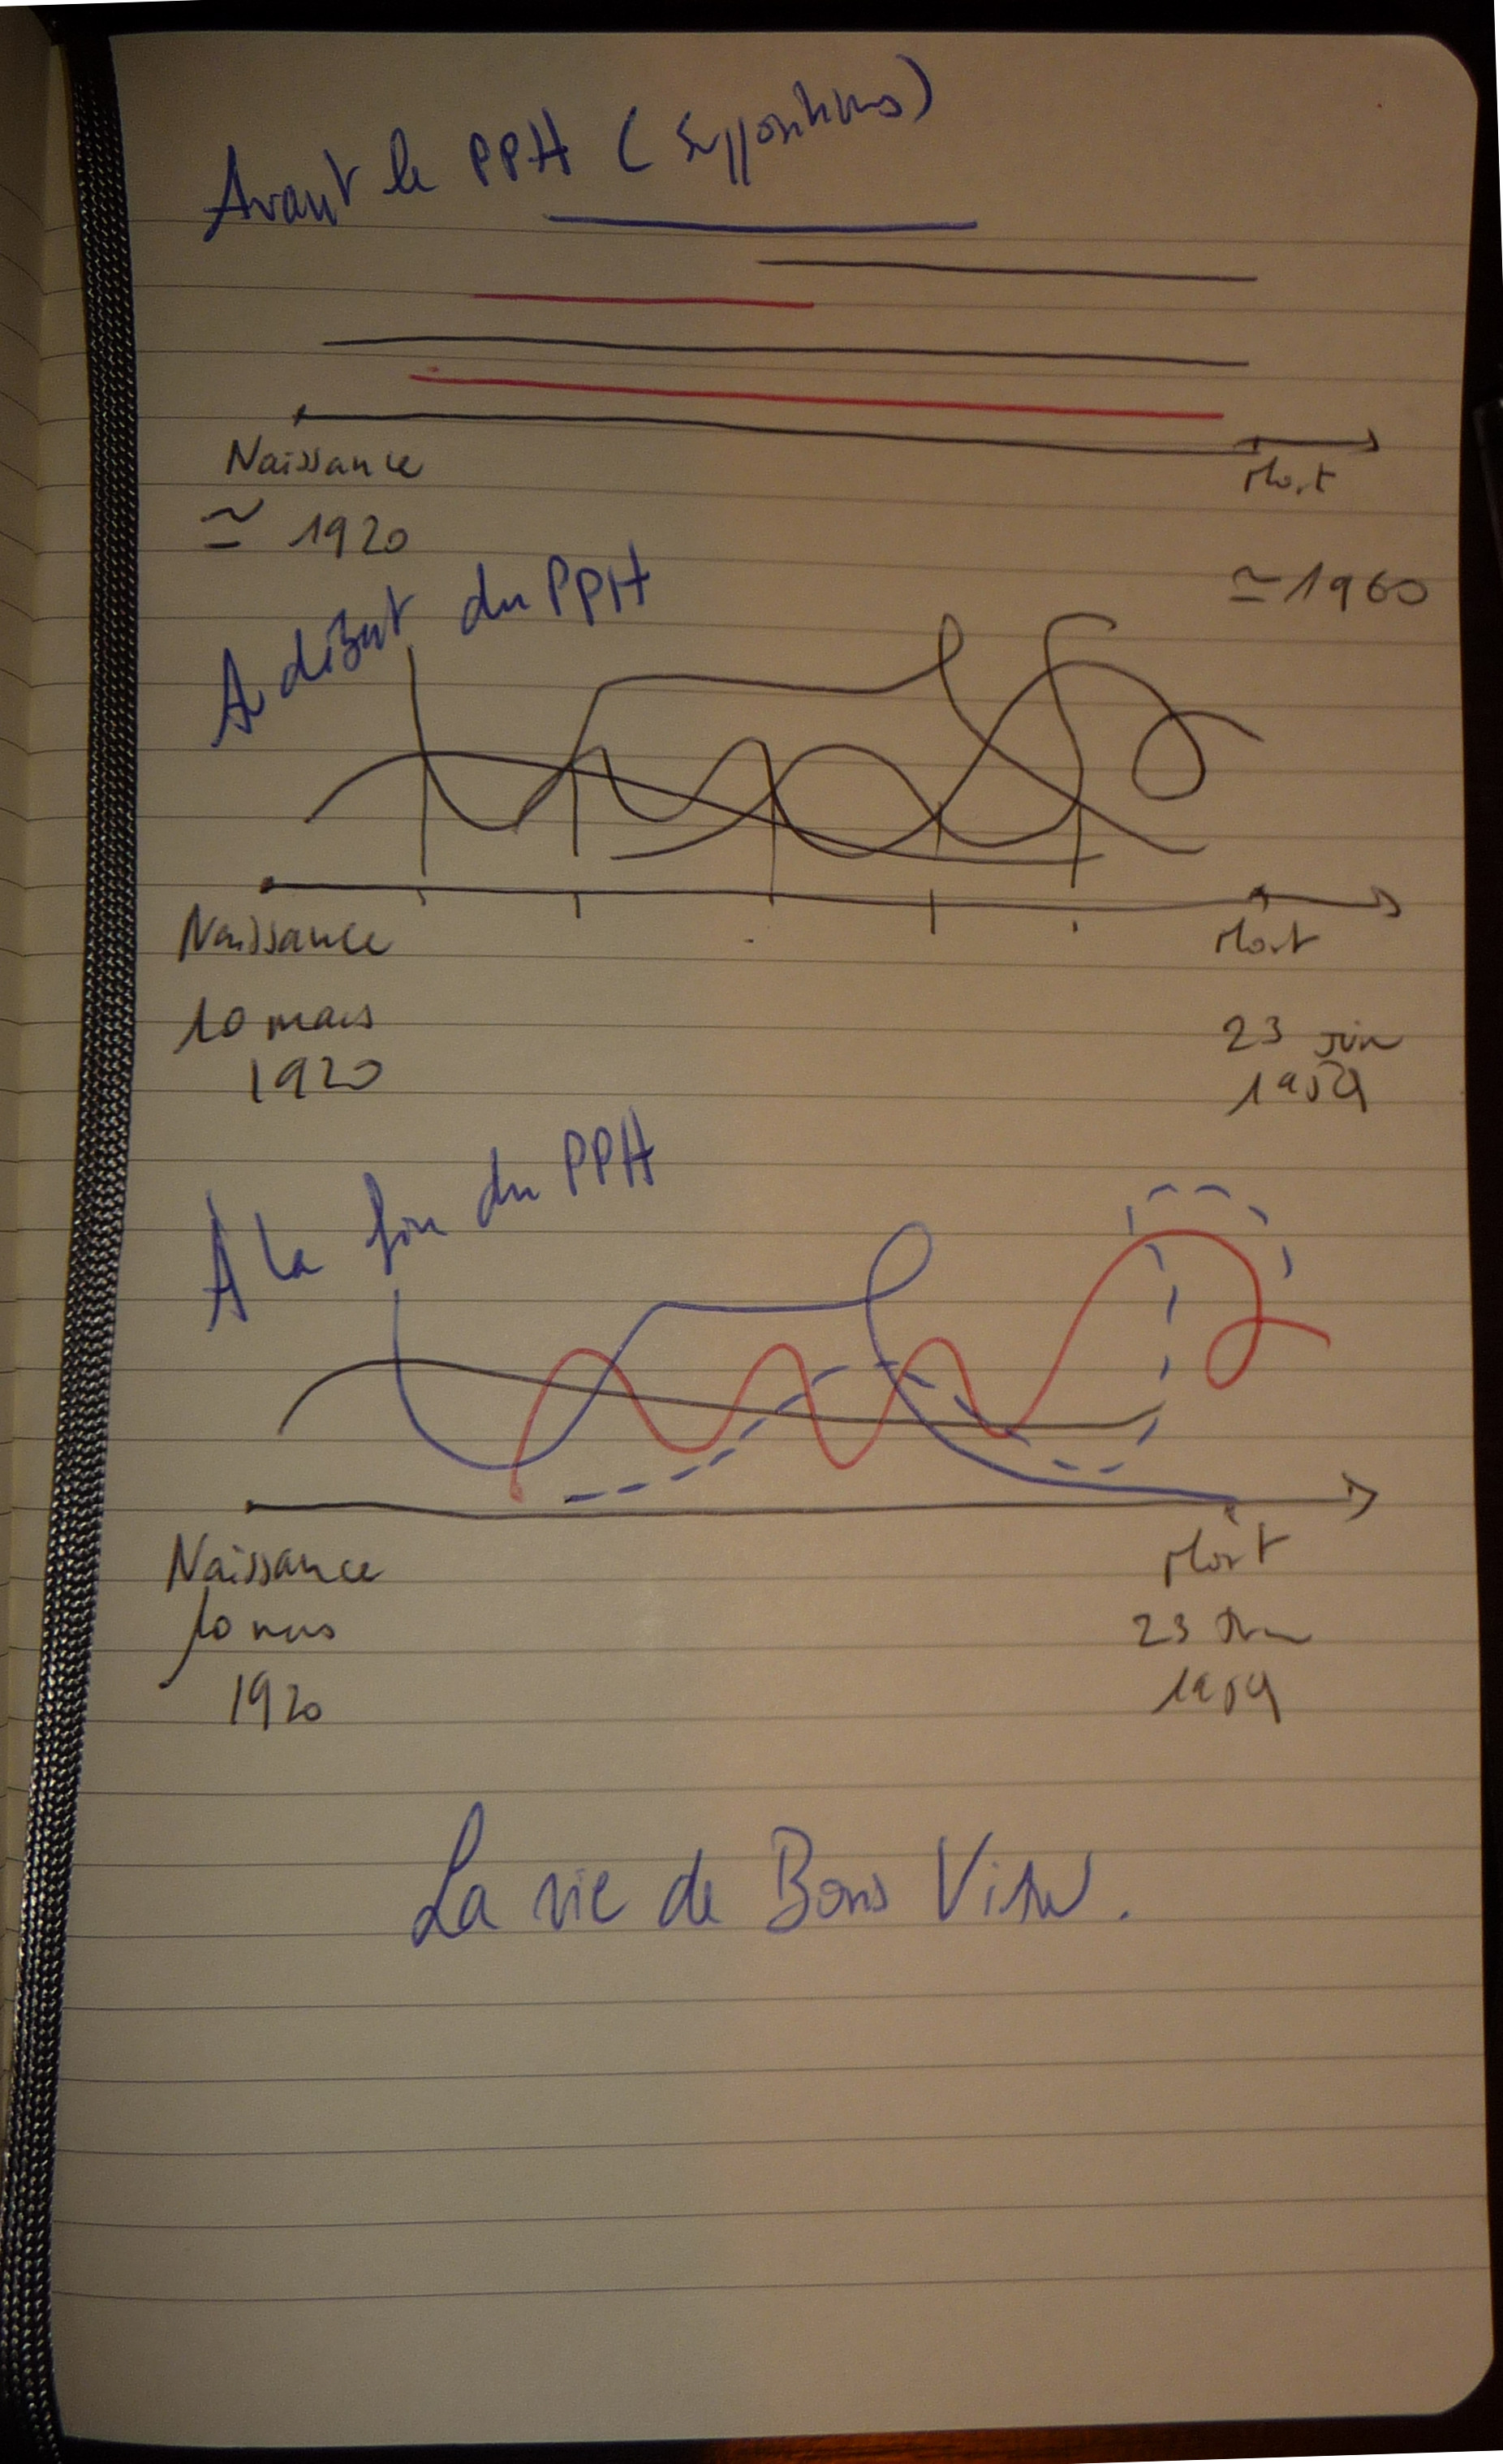
\includegraphics[height=\textheight]{\PIXPATH/carnet}
\caption{Vies de \BV, par Raphaël \bsc{Lizé}}
\label{carnet}
\end{figure}

